\documentclass[UTF8, a4paper]{ctexart}
%\documentclass[utf8]{book}
\usepackage{xeCJK}
\usepackage[colorlinks, linkcolor=red]{hyperref}
\usepackage{xcolor}
\usepackage{listings}
\usepackage{fontspec}
\usepackage{geometry}

% consolas
\newfontfamily\consolas{Consolas}

% green
\definecolor{mygreen}{rgb}{0, 0.6, 0}

% 页边距
\geometry{left=2.5cm,right=2.5cm,top=2.0cm,bottom=2cm}

% 页眉页脚
\pagestyle{empty}

% 代码块设置
% \lstset{
%     basicstyle=\small\consolas, % 代码字体设置
%     columns=flexible,       
%     numbers=none,                                        % 在左侧显示行号
%     frame=single,                                          % 不显示背景边框
%     backgroundcolor=\color[RGB]{245,245,244},            % 设定背景颜色
%     keywordstyle=\color[RGB]{40,40,255},                 % 设定关键字颜色
%     numberstyle=\footnotesize\color{darkgray},           % 设定行号格式
%     commentstyle=\it\color[RGB]{0,96,96},                % 设置代码注释的格式
%     stringstyle=\rmfamily\slshape\color[RGB]{128,0,0},   % 设置字符串格式
%     showstringspaces=false,                             % 不显示字符串中的空格
%     language=bash,                                        % 设置语言
%     breaklines=true, % 自动换行
%     tabsize=4,
% }

\lstset{
    basicstyle=\small\consolas,
    numberstyle= \tiny, 
    keywordstyle= \color{ blue!70},
    %commentstyle=\color{red!50!green!50!blue!50}, 
    commentstyle=\color{mygreen},
    frame=shadowbox, 
    rulesepcolor= \color{ red!20!green!20!blue!20},
    columns=flexible, % 等宽字体
} 

\setCJKmainfont{SimSun}
\title{Deepin Linux 使用笔记}
\author{JackLovel}
\begin{document}

% 段间距
\setlength\parskip{2pt}

% 首行缩进
\setlength\parindent{1em}

\maketitle
\newpage
\tableofcontents

% 章节
\newpage
\setcounter{page}{1} % 从下面开始编码
\chapter{安装}
\section{下载镜像} 
\href{https://mirrors.tuna.tsinghua.edu.cn/}{点击访问清华源官网}

% 可以到\href{https://mirrors.tuna.tsinghua.edu.cn/deepin-cd/}{清华源}下载最新的系统镜像

%\begin{figure}[hbt!] 
%	\centering
%	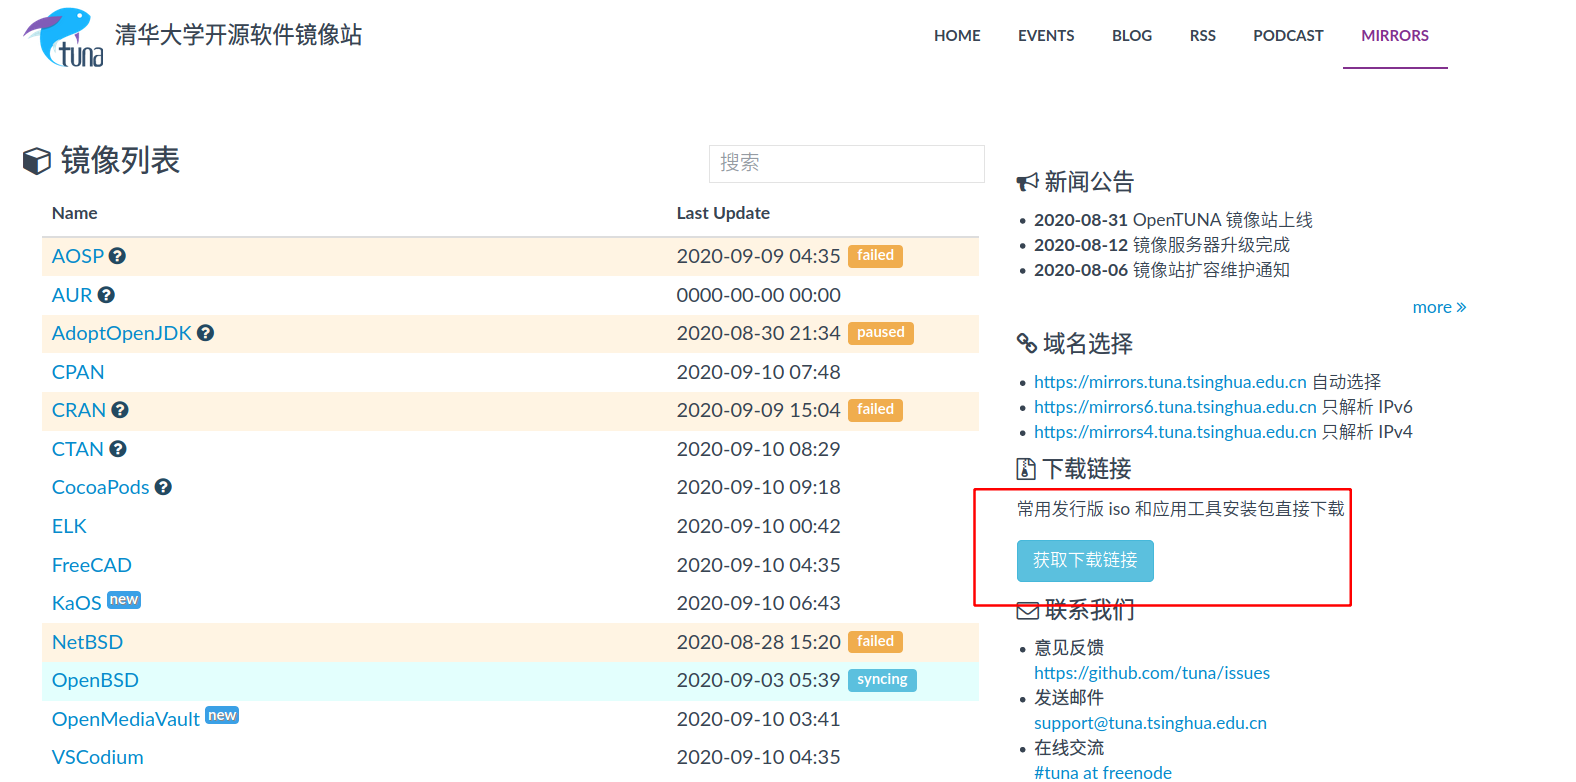
\includegraphics[width=0.49\textwidth]{./img/install/1.png}
%	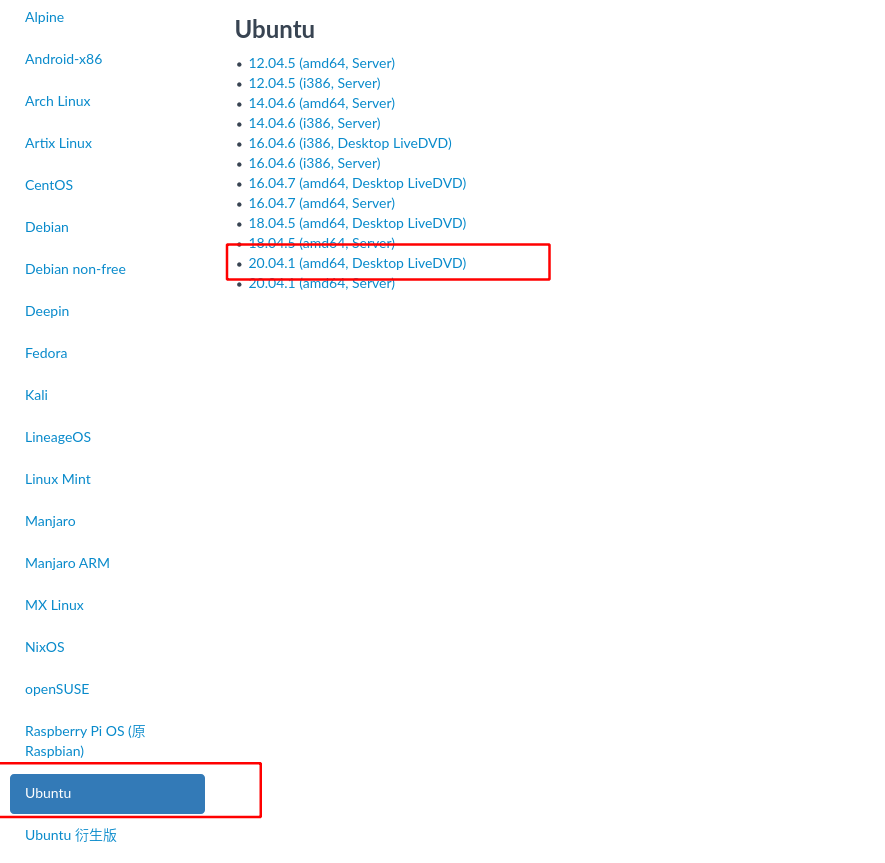
\includegraphics[width=0.49\textwidth]{./img/install/2.png}
%	\caption{镜像下载步骤} %caption是图片的标题
%	\label{fig:ubuntu_download} % 交叉引用
%\end{figure}

\begin{figure}[h!]
	\subfloat[1]{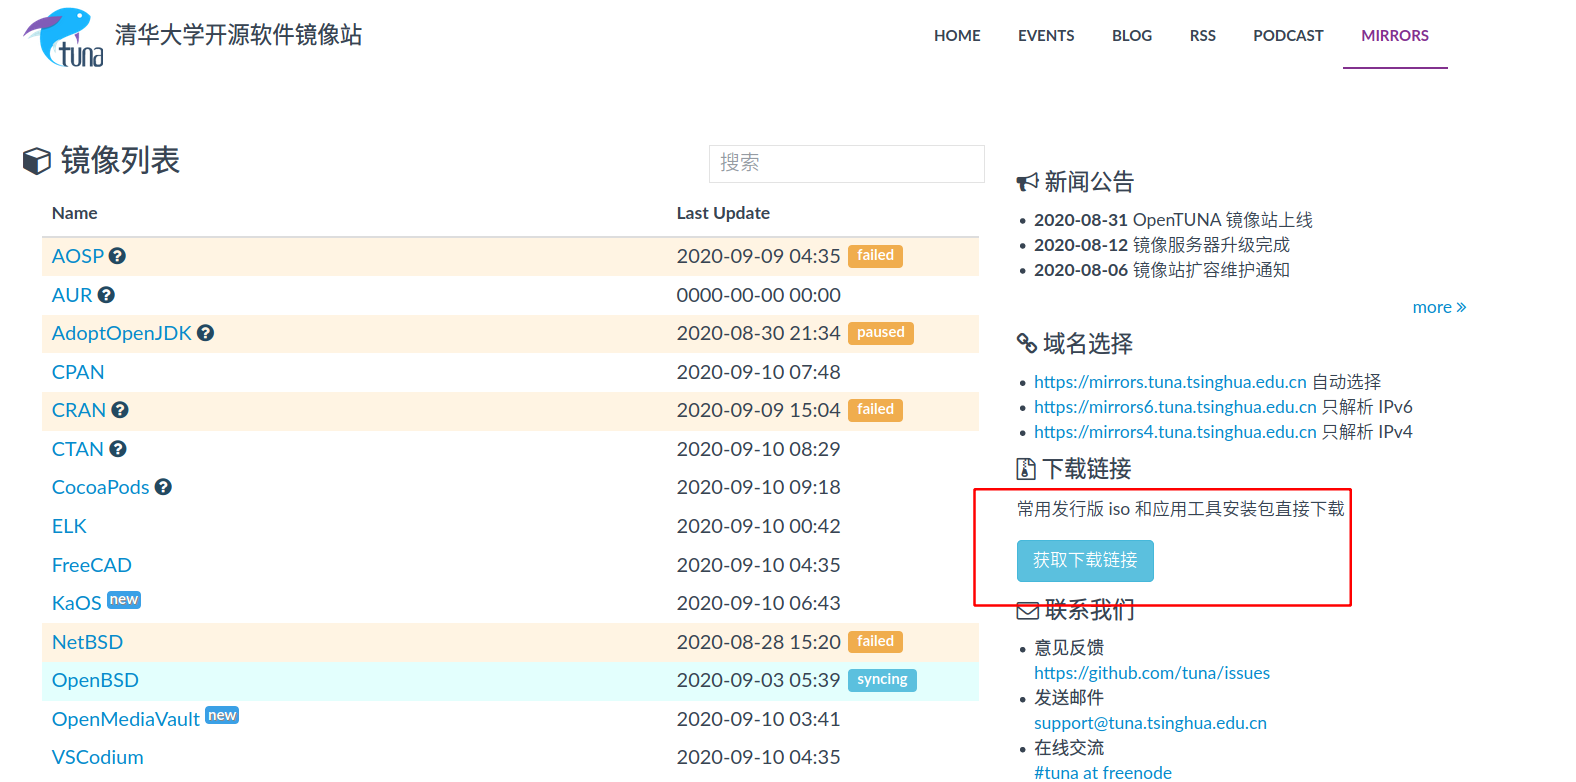
\includegraphics[width=0.6\linewidth]{./img/install/1.png}}\\
	\subfloat[2]{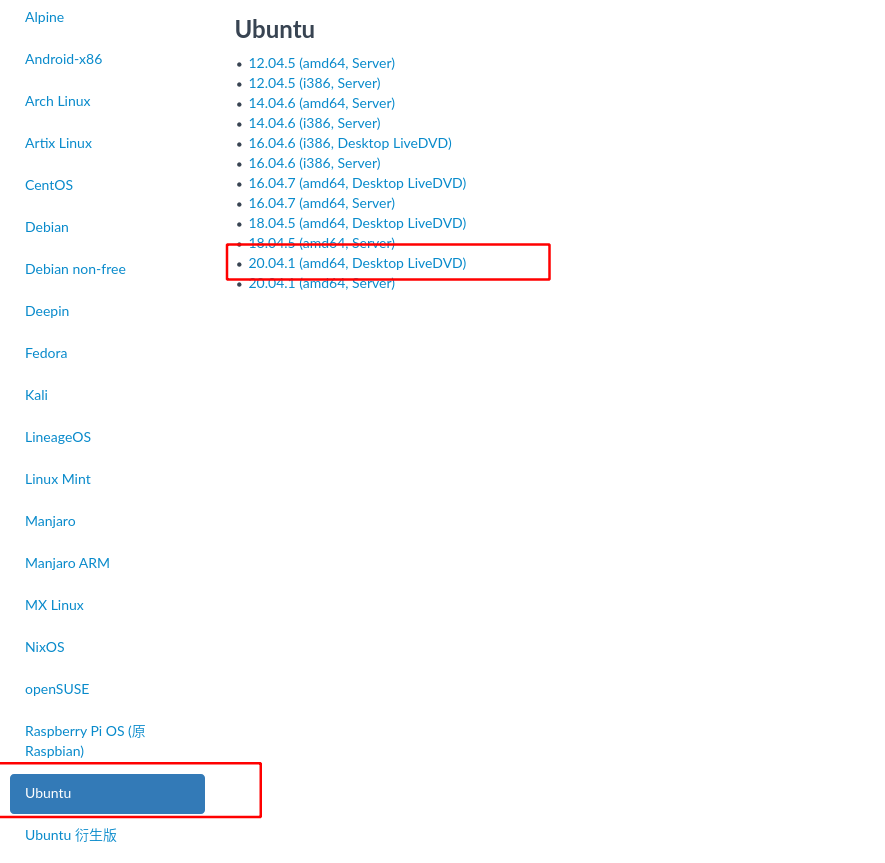
\includegraphics[width=0.6\linewidth]{./img/install/2.png}}
	\caption{镜像下载步骤}
\end{figure}

%\begin{verbatim}
%  https://mirrors.tuna.tsinghua.edu.cn/deepin-cd/
%\end{verbatim}
  
\section{制作启动盘镜像}
制作 linux 启动盘,有很多种方法,下面分别介绍三种:
% window 系统下 
\flushleft
\begin{enumerate}

% liunx 或者 window 下
\item \href{https://www.balena.io/etcher/}{etcher}

比较推荐使用这个软件,来制作系统启动盘,还是比较方便的。

\item 如果在 window 系统下, 可以使用 Rufus, 选好镜像后,分区类型选GPT,刻录模式为DD

Rufus 下载地址:\\
\begin{lstlisting}
 https://share.weiyun.com/51nzNxs
\end{lstlisting}
\item 如果在 linux 系统下,可以使用 dd 命令。
\begin{lstlisting}

$ sudo fdisk -l 

# 我的U盘分区: /dev/sdc
$ umount /dev/sdc1
$ sudo mkfs.vfat /dev/sdc -I

# 我本地 ubuntu 镜像的完整路径:/home/gog/下载/ubuntu-20.04.1-desktop-amd64.iso 
# U盘分区: /dev/sdc
$ cd /home/gog/下载/
$ sudo dd bs=4M if=ubuntu-20.04.1-desktop-amd64.iso of=/dev/sdc status=progress
\end{lstlisting}

\section{分区建议}
这是一个建议的分区,而不是必须的,仅供参考, 这里以 250G 为例:


\begin{tabular}{|l|c|r|}
\hline
 挂载点 & 分区大小(G) & 占比(百分比)\\
\hline
   / & 100 & 40 \\      
\hline
   /home & 100 & 40 \\      
\hline
  交换分区(/swap) & 8 & \\
\hline
  efi分区 & 0.2 & \\
\hline
  /boot & 0.2 & \\
\hline

\end{tabular}
\end{enumerate}


\setlength\parindent{2em}这里分区有几点要说明一下:

\begin{itemize}
\item 根分区和 home分区占大比重,其中 home 你可以在最后分,把剩下的所有的都给它。
\item 这里的换算: 1GB = 1000MB \footnote{在数学换算里 1G = 1024M,但是这里是 1000M}
\end{itemize}

\section{系统配置}
\subsection{更新源}

\begin{itemize}
\item 修改更新源
\begin{lstlisting}
// 以阿里源为例
  
$ sudo cp /etc/apt/sources.list /etc/apt/sources.list.bak  
$ sudo deepin-editor /etc/apt/sources.list

* 将其中的 http://packages.deepin.com/deepin 替换成 http://mirrors.aliyun.com/deepin 
\end{lstlisting}

\item 更新
\begin{lstlisting}
# 更新软件列表
$ sudo apt update  

# 升级软件 
$ sudo apt upgrade 
\end{lstlisting}
\end{itemize}
\section{基本软件的配置}
% zsh
\subsection{zsh}
由于系统原来 bash shell 不怎么好用,所以这里我们推荐使用 zsh \\

安装步骤:
\begin{lstlisting}
$ sudo apt-get install -y zsh
$ sh -c \
 "$(curl -fsSL https://raw.github.com/robbyrussell/oh-my-zsh/master/tools/install.sh)"

# 将 zsh 更改为默认的 shell 
$ chsh -s /bin/zsh 
\end{lstlisting}

安装 percol
\begin{lstlisting}
# 如果 pip 没有安装的话
$ sudo apt install -y python-pip
 
$ sudo pip install percol
$ deepin-editor ~/.zshrc 
\end{lstlisting}

添加下面的内容:
\begin{lstlisting}
function exists { which $1 &> /dev/null }

if exists percol; then
    function percol_select_history() {
        local tac
        exists gtac && tac="gtac" || { exists tac && tac="tac" || { tac="tail -r" } }
        BUFFER=$(fc -l -n 1 | eval $tac | percol --query "$LBUFFER")
        CURSOR=$#BUFFER         # move cursor
        zle -R -c               # refresh
    }

    zle -N percol_select_history
    bindkey '^R' percol_select_history
fi
\end{lstlisting}
\newpage

% emacs 
\subsection{emacs}
下面介绍二种方式安装 emacs:
\flushleft
\begin{enumerate}
% apt 安装
\item 每一种方法,比较简单,但是 emacs 版本还是比较低的。
\begin{lstlisting}
$ sudo apt install -y emacs 

// 查看版本
$ emacs --version  
\end{lstlisting}

% 源码安装
\item 第二种方法,相对于第一种方法来说,略微复杂,比如: 依赖问题;
但是软件版本还是比较高的.

\begin{itemize}
\item 下载源码 \\ 
\begin{lstlisting}
https://www.gnu.org/software/emacs/download.html#gnu-linux
\end{lstlisting}

\item 解压
\begin{lstlisting}
$ tar xvf emacs-26.2.tar.gz  // 解压,并切换到解压后的目录
\end{lstlisting}

\item 安装依赖
\begin{lstlisting}
$ sudo apt-get install build-essential \
  texinfo libx11-dev libxpm-dev libjpeg-dev \
  libpng-dev libgif-dev libtiff-dev libgtk2.0-dev \
  libncurses-dev libxpm-dev automake autoconf 
\end{lstlisting}

\item 编译及安装
\begin{lstlisting}
$ ./configure --with-mailutils 
$ sudo make && sudo make install  
\end{lstlisting}

\item 检测
\begin{lstlisting}
$ emacs --version
\end{lstlisting}

\end{itemize}
\end{enumerate}
\newpage

% java jdk
\subsection{jdk}
这里安装的是 oracle jdk, 所以到 oracle 官网下载 jdk
\begin{itemize}
\item 下载
\begin{lstlisting}
https://www.oracle.com/technetwork/java/javase/downloads/jdk8-downloads-2133151.html
\end{lstlisting}


\item 解压
\begin{lstlisting}
$ tar xvf jdk-1.8.tar.gz
\end{lstlisting}

\item 添加配置,将下面的内容写入 ~/.zshrc 或者 ~/.bashrc
\begin{lstlisting}
export JAVA_HOME= 此处填写jdk的绝对路径
export JRE_HOME=${JAVA_HOME}/jre
export CLASSPATH=.:${JAVA_HOME}/lib:${JRE_HOME}/lib
export PATH=${JAVA_HOME}/bin:$PATH
\end{lstlisting}

\item 检测 
\begin{lstlisting}
$ source ~/.zshrc 

$ java -version 
$ javac 
\end{lstlisting}
\end{itemize}
\newpage

% python
\subsection{python}
\begin{itemize}
\item pip 安装
\begin{lstlisting}
# python2
$ sudo apt install python-pip
$ sudo pip --version

# python3
$ sudo apt install python3-pip
$ sudo pip3 --version
\end{lstlisting}

\item pypi配置
\begin{lstlisting}
$ mkdir ~/.pip
$ cd ~/.pip
$ touch pip.conf
$ deepin-editor ~/.pip/pip.conf 
\end{lstlisting}

然后添加下面的内容:
\begin{lstlisting}
[global]
index-url = http://pypi.douban.com/simple
[install]
trusted-host=pypi.douban.com
\end{lstlisting}

\item ipython
\begin{lstlisting}
# python2
$ sudo apt install -y ipython

# python3
$ sudo apt install -y ipython3 
\end{lstlisting}
\end{itemize}
\newpage

% qt creator
\subsection{qt creator}
\begin{itemize}
\item 下载
\href{http://iso.mirrors.ustc.edu.cn/qtproject/archive/qt/5.8/5.8.0/qt-opensource-linux-x64-5.8.0.run}{qt-opensource-linux-x64-5.8.0.run下载地址}

\item 安装
\begin{lstlisting}
$ chmod +x qt-opensource-linux-x64-5.8.0.run 
$ ./qt-opensource-linux-x64-5.8.0.run 
\end{lstlisting}

\item 解决中文输入
\begin{lstlisting}
$ cd /usr/lib/x86_64-linux-gnu/qt5/plugins/platforminputcontexts

# 我的 qt安装目录: ~/Qt5.8.0
$ cp libfcitxplatforminputcontextplugin.so \
  ~/Qt5.8.0/5.8/gcc_64/plugins/platforminputcontexts

$ cp libfcitxplatforminputcontextplugin.so \
  ~/Qt5.8.0/Tools/QtCreator/lib/Qt/plugins/platforminputcontexts
\end{lstlisting}
\end{itemize}
% docker
% pyenv 

\chapter{其它的软件}
\section{Rust语言}

\begin{itemize}
\item 安装\footnote{官网安装教程:https://www.rust-lang.org/learn/get-started}:
% 代码段
\begin{lstlisting}
$ curl --proto '=https' --tlsv1.2 -sSf https://sh.rustup.rs | sh
\end{lstlisting}
	
\item 配置 Cargo 环境:\\ 
Cargo 用于 包管理和编译程序的工具,将下面的内容添加到 $ \sim $/.bashrc 文件中: \\ 
\begin{lstlisting}
export PATH=$HOME/.cargo/bin:$PATH
\end{lstlisting}
	
\item 使生效
\begin{lstlisting}
$ source ~/.bashrc
\end{lstlisting}

\item 检测
\begin{lstlisting}
# 检测 cargo 版本
$ cargo --version

# 检测 rust 版本
$ rustc --version 
\end{lstlisting}
\end{itemize}
\newpage

\section{Go语言}

\begin{itemize}
\item 安装\footnote{官网安装教程:https://github.com/golang/go/wiki/Ubuntu}:
% 代码段
\begin{lstlisting}
$ sudo add-apt-repository ppa:longsleep/golang-backports
$ sudo apt update
$ sudo apt install golang-go
\end{lstlisting}
	
\item 添加代理
\begin{lstlisting}
$ echo "export GO111MODULE=on" >> ~/.profile
$ echo "export GOPROXY=https://goproxy.cn" >> ~/.profile
$ source ~/.profile
\end{lstlisting}

\item 使生效
\begin{lstlisting}
$ source ~/.profile
\end{lstlisting}
	
\item 检测
\begin{lstlisting}
$ go version
\end{lstlisting}

\item 例子 Gin 网页: 

\begin{lstlisting}
// $ mkdir ginDemo
// $ cd ginDemo 
// $ go mod init gin	
// $ go mod edit -require github.com/gin-gonic/gin@latest	
	
package main

import "github.com/gin-gonic/gin"

func main() {
	r := gin.Default()
	r.GET("/ping", func(c *gin.Context) {
		c.JSON(200, gin.H{
			"message": "pong",
		})
	})
	r.Run() // listen and serve on 0.0.0.0:8080
}

// $ go run demo.go 
\end{lstlisting}
\end{itemize}



\end{document}
